%=============================================================================
% PFPredict Package Appendix
% Copyright (c) 2018. Lester James V. Miranda
%
% This file is part of thesis-manuscript.
%
% thesis-manuscript is free software: you can redistribute it and/or modify
% it under the terms of the GNU General Public License as published by
% the Free Software Foundation, either version 3 of the License, or
% (at your option) any later version.
%
% thesis-manuscript is distributed in the hope that it will be useful,
% but WITHOUT ANY WARRANTY; without even the implied warranty of
% MERCHANTABILITY or FITNESS FOR A PARTICULAR PURPOSE.  See the
% GNU General Public License for more details.
%
% You should have received a copy of the GNU General Public License
% along with thesis-manuscript.  If not, see <http://www.gnu.org/licenses/>.
%
% Created by: Lester James V. Miranda <ljvmiranda@gmail.com>
%=============================================================================

\chapter{The `PFPredict' Package}
\label{AppendixPFPredict}

\par The main workhorse of this research is the PFPredict (\textbf{P}rotein
\textbf{F}unction \textbf{Predict}ion) software package. It is built on top of
Tensorflow and was written using Python 3.6 (also compatible for 2.7). It
contains the core implementation of the mutually-competitive autoencoder
architecture\footnote{
    PFPredict only contains the MC autoencoder. The stacked denoising
    autoencoder is a standard technique that can be implemented solely in
    Keras.
} and its corresponding prediction pipeline.

\section{Dependencies}

\par The table below describes the dependencies for this package. Again,
PFPredict was written in Python 3.6 (with 2.7 compatibility) and was tested
solely on Linux (Ubuntu 16.04) machines.

\begin{table}[!h]
\centering
\caption{Package dependencies}
\label{my-label}
\begin{tabular}{@{}rlp{0.65\textwidth}@{}}
\toprule
Package           & Version & Description                                    \\ \midrule
numpy             & 1.13.0  & matrix and linear-algebra library              \\
scipy             & 0.19.0  & scientific computation library                 \\
tensorflow        & 0.12.1  & tensor computation and neural network library  \\
keras             & 1.2.0   & high-level deep learning framework             \\
scikit-learn      & 0.18.1  & machine learning framework                     \\
scikit-multilearn & 0.0.5   & multilabel learning framework                  \\
future            & 0.16.0  & Python 2 to 3 interface                        \\
pyyaml            & 3.12.0  & easy-parsing of YAML files                     \\
matplotlib        & 1.3.1   & plotting library                               \\ \bottomrule
\end{tabular}
\end{table}


\section{Code Organization and Implementation}

\par There are three main modules in PFPredict: \texttt{utils},
\texttt{extractors}, and \texttt{pipelines}; there is also an auxiliary
\texttt{tests} module for unit tests. The \texttt{utils} module consists of
basic data input/output functionality, preprocessing, and console logging.
Next, the \texttt{extractors} module includes the \texttt{MCAutoencoder} class
for the mutually-competitive autoencoder. Lastly, the \texttt{pipelines} module
includes the \texttt{Pipelines} class where you can define your extractor and
classifier then run it on the data.

\subsection{The \texttt{MCAutoencoder} Class}

\par \texttt{MCAutoencoder} houses the implementation of the
mutually-competitive autoencoder. It inherits from Keras's \texttt{Layer} class
while the internals\textemdash winner-take-all and sparse operations\textemdash
are written in Tensorflow. It also follows \texttt{scikit-learn}'s standard
API: \texttt{fit()}, \texttt{transform(X)}, and \texttt{fit\_transform(X)}. A
UML for this design is seen in Figure \ref{uml:mcae}. 

\par Given a two-dimensional matrix \texttt{X} with each row as a protein
sample and each column a measurement, we can then use the following methods:

\begin{itemize}
    \item \texttt{fit(X)}: train the network using the initialized
        hyperparameters on the training set \texttt{X}. Learns the weight
        parameters of the network.
    \item \texttt{transform(X)}: use the learned weights to transform an input
        \texttt{X} into its latent representation. Returns the extracted
        features.
    \item \texttt{fit\_transform(X)}: higher-level abstraction that calls both
        \texttt{fit(X)} and \texttt{transform(X)} methods successively. Returns
        the extracted features.
\end{itemize}

\begin{figure}[!h]
  \centering
    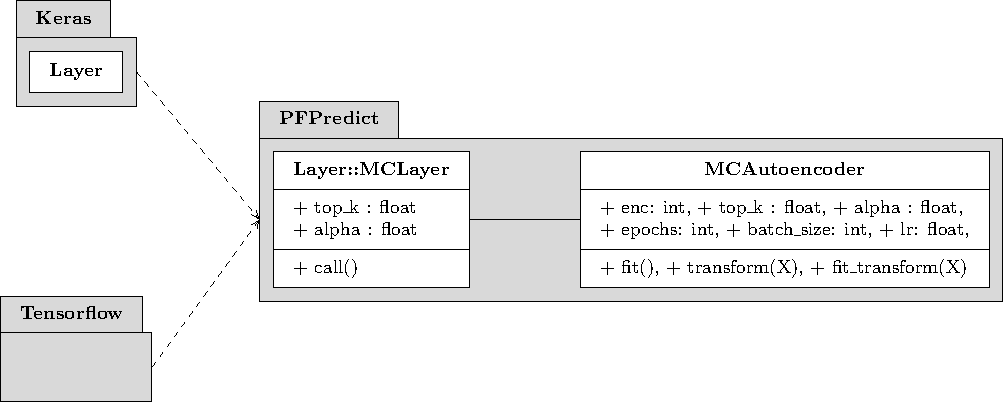
\includegraphics[width=0.85\textwidth]{appendix/uml_mcae}
    \caption{UML Diagram for the \texttt{MCAutoencoder} class}
  \label{uml:mcae}
\end{figure}

\par The main idea is to first initialize the \texttt{MCAutoencoder} class by
setting the hyperparameters, call the \texttt{fit(X)} method to the training
set, then call the \texttt{transform(X)} method to both training and test (or
validation) sets. The \texttt{transform(X)} method returns the extracted
features that we can now use for classification. The code sample below
illustrates this process.

\lstset{backgroundcolor=\color{gray!30}, basicstyle=\ttfamily,
breaklines=true}
\begin{lstlisting}[style=mypython, caption=Minimal example for extracting
protein features]
from pfp.extractors import MCAutoencoder
from pfp.utils import load_dataset

# Load Yeast dataset (we will not use the labels: unsupervised)
X_train, y_train, X_test, y_test = load_dataset('yeast', scale=True)
# Initialize the autoencoder with hyperparameters
feature_extractor = MCAutoencoder(enc=500, top_k=0.6, alpha=10.0)
# Fit model and learn network weights
feature_extractor.fit(X_train)
# Transform raw attributes into new features
X_train_new = feature_extractor.transform(X_train)
X_test_new = feature_extractor.transform(X_test)
\end{lstlisting}

\subsection{The \texttt{Pipelines} Class}

\par In order to run the experiments with ease, we designed a
\texttt{Pipelines} class that abstracts away the \texttt{MCAutoencoder} and
classifier. It takes a dataset, a feature extractor, and a multilabel
classifier as its input, and runs the whole prediction pipeline for a given
number of trials. It then returns a dictionary of scores for model evaluation.
The classifier object is obtained from the \texttt{scikit-multilearn}
library.\footnote{The author is also a collaborator in this project. Please see
\url{https://github.com/scikit-multilearn} for more information}

\begin{lstlisting}[style=mypython, caption=Minimal example for the prediction
pipeline]
from pfp.extractors import MCAutoencoder
from skmultilearn.problem_transform import BinaryRelevance
from sklearn.svm import SVC
from pfp.utils import load_dataset
from pfp.pipelines import Pipelines

# Load Yeast dataset (we will not use the labels: unsupervised)
yeast  = load_dataset('yeast', scale=True)
# Initialize the autoencoder with hyperparameters
mcae = MCAutoencoder(enc=500, top_k=0.6, alpha=10.0)
# Initialize the BR-SVM classifier
brsvm = BinaryRelevance(classifier=SVC(), require_dense=[False, True])
# Put extractor and classifier to pipeline and run
pipeline = Pipelines(extractor=mcae, classifier=brsvm, dataset=yeast)
scores = pipeline.run(trials=10)
\end{lstlisting}

\section{Miscellaneous Information}

\par This package is hosted in
\url{https://github.com/ljvmiranda921/pfpredict}, but, at this time of writing,
currently set to private. Continuous integration (CI) and deployment is set up
using TravisCI (\url{https://travis-ci.org/}), and the unit tests were written
using the \texttt{unittest} module.
